\documentclass[12pt,a4paper,titlepage]{article}
% para que '{' y '}' se puedan imprimir en texttt
\usepackage[T1]{fontenc}
\usepackage[utf8]{inputenc}
\usepackage[spanish]{babel}
% acentos en la bibliografía
\usepackage{csquotes}

% para que el índice y las referencias tengan enlaces
\usepackage[hidelinks]{hyperref}
% bibliografía (style=ieee: referencias por orden de aparición)
\usepackage[backend=biber, style=ieee]{biblatex}
\addbibresource{proyecto.bib}
% imágenes
\usepackage{graphicx}
% diagramas (https://texample.net/tikz/examples/er-diagram/)
\usepackage{tikz}
% \usetikzlibrary{er, positioning}
\usetikzlibrary{er, positioning, babel, shapes.multipart}
% diagrama gantt
\usepackage{pgfgantt}

% mostrar colores
\usepackage{xcolor}
% (revisar: https://github.com/denki/listings-rust)
% mostrar bloques de código
\usepackage{listings}
\renewcommand{\lstlistingname}{Ejemplo}
\renewcommand{\lstlistlistingname}{Ejemplos de código}
% estilo de código para JavaScript
% (https://www.youtube.com/watch?v=qxkQgG1Y0bY)
\lstdefinestyle{javastyle}{
    basicstyle=\ttfamily\small,
    breaklines=true,
    commentstyle=\color[HTML]{2b922c},
    keywordstyle=\color[HTML]{6b2eff},
    stringstyle=\color[HTML]{ac2f38},
    showstringspaces=false,
    numbers=left,
    numberstyle=\ttfamily\footnotesize,
    stepnumber=1
}

% comandos específicos del documento
\newcommand\projectname{$\Delta$chan}
% \newcommand\projectname{My-chan}

\title{\projectname\\\bigskip\normalsize{Proyecto fin de ciclo\\Desarrollo de Aplicaciones Multiplataforma}}
\author{Alfredo Rodríguez Gracía}
\date{21 de mayo de 2021\\\bigskip\scriptsize{última revisión\\\today}}

\begin{document}
    % - portada 
    \maketitle
    % - índice 
    \tableofcontents
    \vspace{\fill}
    % - licencia (CC-BY)
    \begin{center}
        
\includegraphics[width=0.15\textwidth]{media/cc-by-large.png}

        \small{Obra bajo licencia de \textit{Creative Commons} Reconocimiento 4.0 Internacional.}
    \end{center}
    \newpage

    \section{Descripción del proyecto}

    %Breve descripción del proyecto indicando qué es lo que hace, para qué sirve y si tiene futuros usos con pequeñas modificaciones.

    %\bigskip\hrule\bigskip

    {\projectname} (pronunciado como \textit{dichan}) es un proyecto de tablón de imágenes \cite{wiki:imageboard}, centrado en el anonimato y la libertad de expresión \textit{on-line}, dónde los usuarios pueden subir imágenes y vídeos cortos para iniciar un debate. Está inspirado en otros tablones existentes como \emph{4chan} y \emph{2channel}, sitios que, a pesar del enorme auge de las redes sociales, siguen siendo el refugio de muchos internautas hoy en día.

    Un tablón de imágenes (también conocido por su nombre en inglés: \textit{imageboard}) es un tipo de página web anónima donde la publicación de imágenes y pequeños vídeos cobra una gran importancia. Los primeros tablones de imágenes fueron creados en Japón a finales de los 90, y se basan en el concepto de los foros de texto. En términos generales ambos comparten la misma estructura, incluyendo la separación de los debates (\textit{threads}) de diferentes temáticas en secciones, llamadas tablones o \textit{boards}. Sin embargo, los \textit{threads} en los \textit{imageboards} pueden llegar a ser mucho más esporádicos que en los foros convencionales, donde el tiempo de vida de uno puede ser inferior a varias horas. Los tablones de imágenes más populares en occidente tienden a estar relacionados en su mayoría con la cultura japonesa, como son la temática del \emph{anime} y \emph{manga}. Sin embargo, en Japón son más populares y sus tópicos abarcan una gran variedad de temas.

    \begin{figure}[ht]
        \centering
        \caption{Vista del board \texttt{/w/} de \textit{4chan}}\bigskip
        \label{4chan:board}
        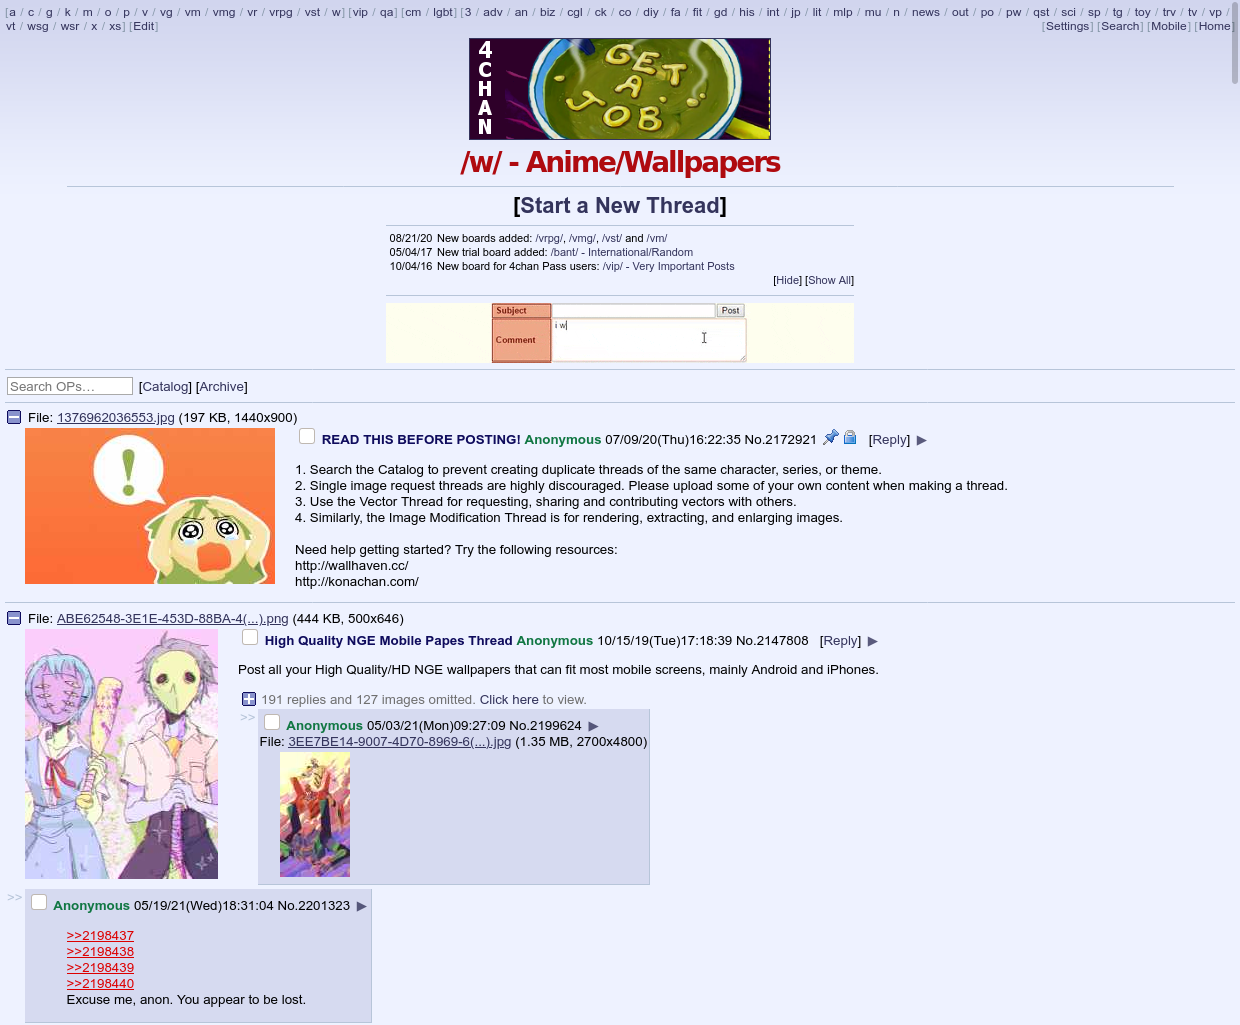
\includegraphics[width=1.0\textwidth]{media/4chan-board.png}
    \end{figure}

    El proyecto {\projectname} intenta emular a estos tablones haciendo muy sencillo que cualquiera que lo desee pueda montar su propia instancia en un equipo, incluso con muy pocos recursos. La estructura de la página es muy simple, consta principalmente de dos partes bien diferenciadas: la portada, donde se visualizará la lista de \textit{boards} activos en la página; y los \textit{boards} en sí, cada uno de su temática particular y limitado a nueve páginas de contenido. Cada página de un \textit{board} contendrá cinco \textit{threads} ordenados por fecha de actualización más reciente, es decir, en el primer puesto de la primera página se colocará el \textit{thread} que ha recibido el último comentario y en el último puesto de la novena página estará el \textit{thread} que ha pasado más tiempo sin comentarios. En el momento que un usuario decida abrir un nuevo \textit{thread} ese último se borrará y el nuevo aparecerá en el primer puesto. De esta forma se consigue ese dinamismo tán característico de los \textit{imageboards} dónde tienes la certeza de que lo primero que ves al entrar es de lo que se está hablando actualmente, es el tema del momento.

    La intención del proyecto mira hacia un futuro colaborativo, donde muchas personas puedan aportar sus opiniones y mejoras al mismo. Este es el motivo por el que se publica bajo la \emph{GNU General Public License version 3} \cite{gnugplv3}, para garantizar que forme parte del movimiento del \emph{software libre} definido por \textcite{libresoftwaredefinition}. El código fuente será accesible desde un repositorio \emph{Git} de libre acceso, donde cualquier persona podrá proponer cambios a través de los procedimientos establecidos. De esta forma también es posible que surjan \textit{forks} \cite{wiki:fork} donde, utilizando este proyecto como base, cualquiera puede cambiar radicalmente el propósito original y aportar un enfoque completamente diferente.

    \subsection{Partes del proyecto}

    El proyecto consta de tres partes muy bien diferenciadas: la \textbf{página web}, la cual constituye el \textit{frontend}, desarrollada utilizando \emph{HTML5}, \emph{CSS3} y \emph{ECMAScript 6} (\emph{JavaScript}), es la encargada de lidiar cara a cara con el usuario final, mostrar los resultados de las llamadas a la \emph{API} y distribuir esas respuestas adecuadamente en la interfaz gráfica (\emph{GUI}); la \emph{\textbf{API}}, una de las dos partes del \textit{backend}, desarrollada utilizando el lenguaje \emph{Python} utilizando la librería \textit{Flask}, es la intermediaria entre la web y los datos almacenados, ofreciendo un estándar a la hora de consultar y modificar la información ofrecida por los usuarios; y la segunda parte del \textit{backend} es la \textbf{base de datos} que, corriendo sobre un servidor \emph{MariaDB}, almacenará toda la información de la aplicación en tablas relacionadas para poder acceder a ella de la manera más eficiente posible, garantizando siempre la integridad y la alta disponibilidad de los datos. Observando la figura \ref{project:schema} se puede observar de forma gráfica cómo se relacionan entre sí estas tres partes.

    \begin{figure}[ht]
        \centering
        \caption{Vista del la portada de \textit{2chan}}\bigskip
        \label{2chan:home}
        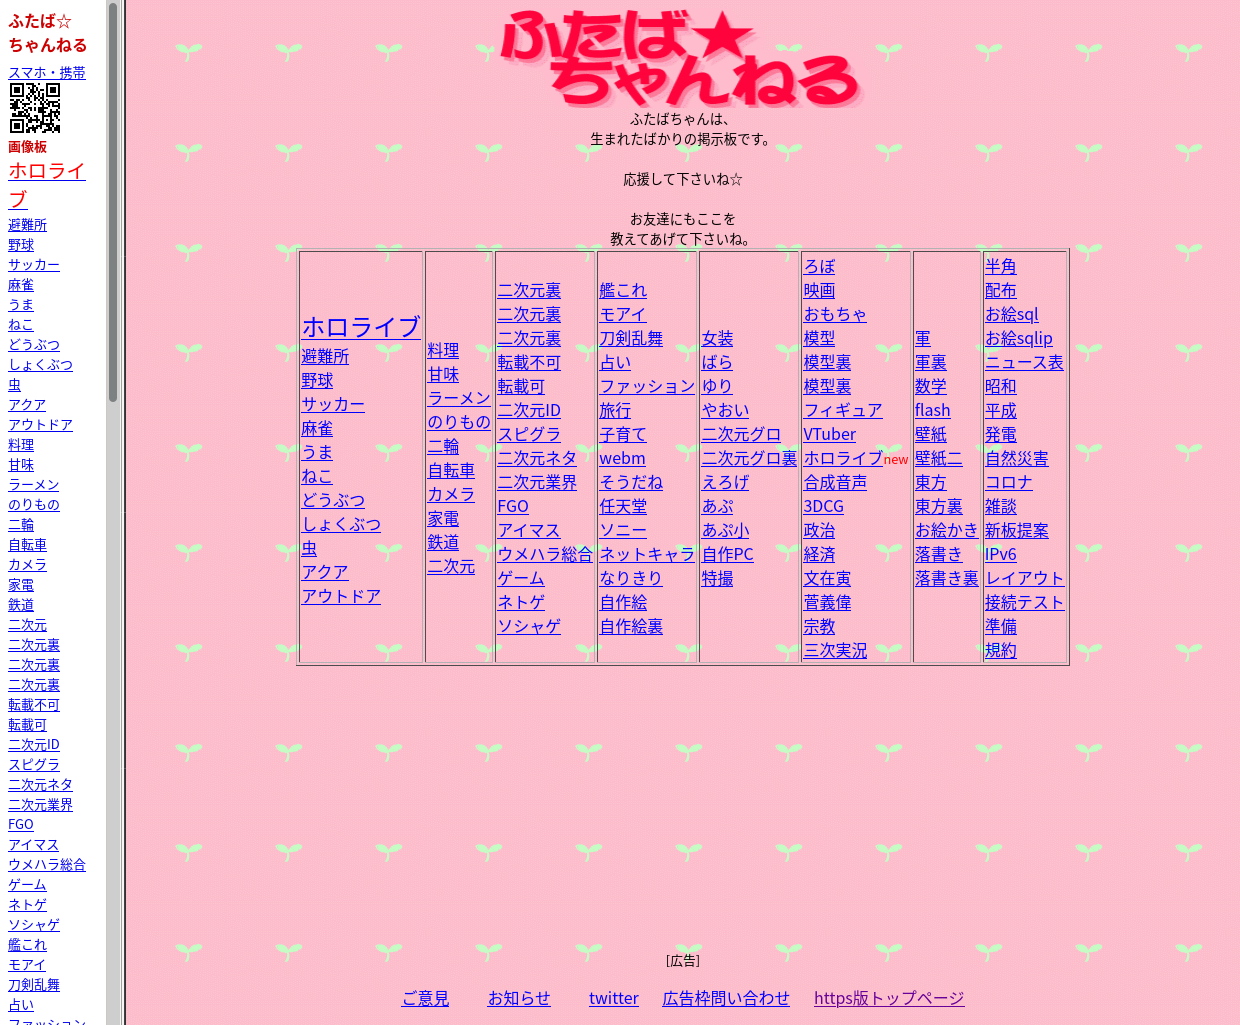
\includegraphics[width=1.0\textwidth]{media/2chan-home.png}
    \end{figure}

    La grán ventaja de utilizar un \emph{API} en el \textit{backend} es que, de esta forma se abre la posibilidad a la aparición de clientes programados por terceros que interactúen con los datos a través de un interfaz común para todos ellos. Haciendo muy portable el proyecto hacia nuevos entornos, como por ejemplo, en forma de app movil, aplicación de escritório u otras interfaces web. Asimismo, el hecho de independizar por completo el cliente del servidor permite que futuras versiones puedan prescindir de alguna de las partes con mucha facilidad y re-implementarla al gusto, facilitando al máximo la re-utilización del código.

    \section{Ámbito de implantación}

    % Deberá describirse el lugar (empresa, organización, sector...) en el que se implantará el proyecto y con qué objetivo, además de indicar a quién va dirigida la aplicación, es decir, identificar quién o quiénes serán los principales usuarios de la misma.

    % \bigskip\hrule\bigskip

    {\projectname} será administrado por una organización sin ánimo de lucro (\textit{The {\projectname} Foundation}), creada específicamente con la finalidad de asegurar la libertad, independencia y neutralidad del proyecto, así como mantenerlo ajeno a todo interés económico, político y personal que pueda derivar de una administración centrada en una única o un reducido número de personas. Imitando así modelos como los implementados en \emph{Wikimedia} \cite{wikimedia:about} o \emph{The Internet Archive} \cite{internetarchive:about}. Esta será la encargada tanto de la parte financiera, administrando las donaciones que se puedan recibir por parte de los usuarios, como la parte tecnológica, ofreciendo al proyecto de la infraestructura física y el mantenimiento necesario para asegurar su correcto funcionamiento.
    
    El objetivo final pasa por establecer un lugar de debate e intercambio de opiniones abierto, libre y neutral; donde cada usuario pueda encontrar su rincón y hablar de lo que le apetezca con personas que comparten sus mismos gustos y aficiones. Y al mismo tiempo ofrecer espacios donde posiciones opuestas se enfrenten para que eventualmente se alcance un consenso común y beneficioso para ambas partes.
    
    Este proyecto va dirigido a usuarios que les importan más las ideas --el debate en sí-- y no las personas que sostienen esas ideas, gente de todas las edades que quiera compartir sus opiniones y experiencias con una gran comunidad de distribuida por todo el mundo. El anonimato hace que la gente se pueda expresar sin tapujos y sin esperar consecuencias en el ámbito personal, instigadas por lo que uno piensa.

    \section{Recursos de \textit{hardware} y \textit{software}}

    % Se describirán los requisitos mínimos y los requisitos recomendados de \textit{hardware}, tanto para el desarrollo de la aplicación, como para su instalación y ejecución.

    % Se describirán las necesidades de \textit{software} requeridas para el desarrollo de la aplicación.

    % \bigskip\hrule\bigskip

    Puesto que {\projectname} es un \emph{aplicación web} existen tres escenarios a tratar con respecto a los requisitos de \textit{hardware} y software: \textbf{desarrollo}, \textbf{despliegue} e \textbf{instalación por parte del usuario}. Inicialmente se pretende que en cualquier de ellos, estos recursos, sean lo más limitados y gratuitos posibles haciendo que el proyecto pueda ser accesible por cualquiera sin importar la calidad del \textit{hardware} disponible.

    \subsection{Requisitos de desarrollo}

    Los requisitos para el desarrollo de este proyecto no son para nada exigentes, todas las partes se pueden montar e interconectar en un mismo equipo con, prácticamente, cualquier especificación de \textit{hardware}. Unos requisitos mínimos podrían ser, un CPU de al menos cuatro núcleos y 2.0GHz de frecuencia, con al menos 4 GB de memoria \textit{RAM}, 10 GB de espacio libre en el dísco duro y, como requisito extra, es indispensable una conexión estable a internet en el puesto de trabajo, a ser posible de 50Mbps o superior. Alternativamente se recomienda lo siguiente: CPU con más de cuatro núcleos y frecuencia mínima cercana a 2.0GHz, 16Gb de \textit{RAM} y 50Gb de espacio libre en \textit{SSD}.

    Además del \textit{hardware}, los siguientes programas son necesarios para poder montar un entorno de desarrollo adecuado y funcional (todos ellos en sus versiones más recientes): un servidor de base de datos \emph{MariaDB} o \emph{MySQL}, para poder ejecutar consultas \emph{SQL} contra él en el entorno local, que gracias a \textit{Docker} \cite{docker:overview} se podrá emular de la forma más similar como se realizarán una vez se haya desplegado toda la infraestructura; un servidor \textit{HTTP}, también ``\textit{dockerizado}'', como puede ser \emph{NGINX} o \emph{Apache2}; y, por último será necesario un gestor de versiones como \textit{Git} encargado de gestionar las versiones y coordinar a las diferentes personas encargadas del desarrollo. Por otra parte, se recomiendan algunos programas opcionales que quedan a elección del desarrollador, com puede ser, un editor de código adaptado para las diferentes tecnologías y lenguajes utilizados en el proyecto (\emph{Visual Studio Code OSS}, \emph{Atom}, \emph{Geany}\dots); un cliente de bases de datos como \emph{DBeaver} o \emph{MySQL Workbench}, para administrar de manera más sencilla la base de datos en las fases más tempranas del desarrollo. Y como apunte final sería aconsejable realizar todo el proceso de desarrollo sobre una distribución de \emph{GUN/Linux} para simplificar al máximo la portabilidad al entorno del servidor cuando el proyecto se pase a fase de \emph{producción}.

    \subsection{Requisitos de despliegue}

    El despliegue de la aplicación en el ámbito del servidor está pensado para realizarse en contenedores de \textit{Docker} sobre un SO \emph{GNU/Linux}, haciendo el entorno lo más ligero y portable posible, permitiendo una grán escalabilidad de cara al futuro. Al principio, el proyecto se podrá montar sobre una única máquina, y gracias a estar pensado para ser muy ligero, esta máquina no requerirá de unas características desmesuradas. Se podrá desplegar el proyecto en cualquier máquina virtual en la nube, por ejemplo en una instancia de \textit{Amazon Web Services} (\textit{AWS}), \textit{Google Cloud}, \textit{Digital Ocean} o \textit{Linode}; pero también en cualquier máquina virtual en un servidor propio. Además, si se prefiere, se puede instalar el servicio en una máquina física o distribuirlo por un entorno de varios servidores, en caso de prever grandes picos de tráfico. En cuanto al \textit{hardware} (virtualizado o físico) mínimo se necesitan al menos las siguientes características: un CPU de al menos cuatro núcleos y 2.0GHz de frecuencia, memoria \textit{RAM} de 8Gb o superior, 100Gb de espacio libre en dísco duro y, sobre todo 100Mbps de conexión estable a internet. Pero, sin embargo, se recomienda: CPU con más de cuatro núcleos y frecuencia mínima cercana a 2.0GHz, 32Gb de \textit{RAM}, 500Gb de espacio libre en \textit{SSD} y conexión redundante y estable de al menos 600Mbps.

    Tanto el diseño como el desarrollo de la base de datos se realizarán pensando en un servidor \emph{MariaDB}, dejando así la puerta abierta a una mayor compatibilidad con \emph{MySQL} y otras tecnologías similares. Estará pensada para ser lo más ligera posible, permitiendo que pueda ser alojada en el mismo equipo que el servidor \emph{HTTP}. este se espera que sea un \textit{NGINX} preferiblemente, o un \textit{Apache2} como segunda opción, los dos excelentes servidores libre utilizados tanto a nivel personal como profesional. Es importante hacer notar que las versiones de estos programas en el ámbito del servidor se deben tomar con mucha cautela, y se suelen escoger las marcadas con el \textit{tag} \textit{LTS} (\textit{Long Term Support}) para no sufrir cambios derivados de alguna futura actualización que puedan afectar al correcto funcionamiento de la aplicación.

    \subsection{Requisitos de instalación por parte del usuario}

    Al ser una aplicación web no requiere de una instalación, como tal, en el equipo del usuario final. Pero si que necesita de unos requisitos mínimos que vienen definidos por las tecnologías utilizadas en la parte del \textit{frontend}. Por ejemplo, el usuario necesita tener instalado en su equipo por lo menos un navegador web que sea capaz de soportar código \emph{ECMAScript 6} para que el \emph{JavaScript} pueda funcionar sin ningún impedimento. Los navegadores más modernos, en sus versiones más actualizadas, con motores como \emph{Gecko} (\emph{Mozilla Firefox}) o \emph{Webkit} (\emph{Google Chrome}, \emph{Opera}, \emph{Brave}\dots) son perfectamente compatibles con esta reciente tecnología.

    Con respecto a los requisitos \textit{hardware}, no se requiere nada fuera de lo común, se considera que hoy en día todo dispositivo (\textit{PC} o \textit{smartphone}) posee las capacidades básicas para abrir un navegador, acceder a una página web y leer texto, visualizar imágenes o pequeños vídeos.

    \section{Temporalización del desarrollo}

    % Deben describirse las distintas actividades necesarias para desarrollar el proyecto, asignarles un tiempo a cada una de ellas y construir los dos diagramas completos.

    % \bigskip\hrule\bigskip

    Lista de tareas a realizar y cuanto tiempo conlleva cada una\footnote{Nótese que las tareas de diseño de la base de datos y definición de los \textit{endpoints} de la \textit{API} no se tienen en cuenta en la planificación temporal, porque ya están realizadas en este documento.}.

    \begin{enumerate}
        \renewcommand{\theenumi}{\Alph{enumi}} % abc enumeration
        \item (2d\footnote{Unidades de tiempo en días.}) \textit{Setup} del entorno de desarrollo (\textit{hardware} y \textit{software}).
        \item (5d) Diseño de \textit{mockups} para las pantallas de la web.
        \item (4d) Desarrollo y testeo de la base de datos.
        \item (7d) Desarrollo y testeo de los \textit{endpoints} de la \textit{API}.
        \item (3d) Desarrollo y testeo de la conexión de la \textit{API} con la base de datos.
        \item (3d) Desarrollo y testeo de la estructura y funciones básicas de la web.
        \item (4d) Desarrollo y testeo de la conexión de la web con la \textit{API}.
        \item (3d) Implementación de los estilos en la web.
        \item (2d) Internacionalización de los textos de la web.
        \item (5d) Setup del entorno del servidor (\textit{hardware} y \textit{software}).
        \item (5d) Despliegue y publicación de la aplicación en el entorno del servidor.
        \item (7d) Redacción de la documentación del proyecto.
    \end{enumerate}

    \begin{figure}[ht]
        \centering
        \caption{Diagrama de Gantt}
        \label{diagram:gantt}
        \begin{ganttchart}[vgrid, x unit=0.50cm, y unit chart=0.3cm, bar height=1.0, bar top shift=-0.0, title height=0.45]{1}{23}
            \gantttitlelist{1, ..., 23}{1} \\
            \ganttbar{\footnotesize{A}}{ 1}{ 2} \\
            \ganttbar{\footnotesize{B}}{ 1}{ 5} \\
            \ganttbar{\footnotesize{C}}{ 3}{ 6} \\
            \ganttbar{\footnotesize{D}}{ 3}{ 9} \\
            \ganttbar{\footnotesize{E}}{10}{12} \\
            \ganttbar{\footnotesize{F}}{ 6}{ 8} \\
            \ganttbar{\footnotesize{G}}{10}{13} \\
            \ganttbar{\footnotesize{H}}{14}{16} \\
            \ganttbar{\footnotesize{I}}{17}{18} \\
            \ganttbar{\footnotesize{J}}{ 1}{ 5} \\
            \ganttbar{\footnotesize{K}}{19}{23} \\
            \ganttbar{\footnotesize{L}}{14}{20} \\
        \end{ganttchart}
    \end{figure}

    \begin{figure}[ht]
        \centering
        \caption{Diagrama PERT}\bigskip
        \label{diagram:pert}
        \begin{tikzpicture}[scale=0.7, every node/.style={transform shape}, trinode/.style={circle split, draw, path picture={\draw (path picture bounding box.center)--(path picture bounding box.south);}}]
            % level 0
            \node[trinode] (n1) {1\nodepart{lower} 00\ \ 00};
            % level 1
            \node[trinode, below right=2.15of n1] (n2) {2\nodepart{lower} 02\ \ 02};
            \draw[->, very thick] (n1)--(n2) node[midway, above right]{A(2)};
            \node[trinode, below=of n1] (n3) {3\nodepart{lower} 05\ \ 06};
            \draw[->] (n1)--(n3) node[midway, right]{B(5)};
            \node[trinode, below left=4.0of n1] (n4) {4\nodepart{lower} 05\ \ 18};
            \draw[->] (n1)--(n4) node[midway, above left]{J(5)};
            % level 2
            \node[trinode, below right=2.15of n2] (n5) {5\nodepart{lower} 06\ \ 09};
            \draw[->] (n2)--(n5) node[midway, above right]{C(4)};
            \node[trinode, below=of n2] (n6) {6\nodepart{lower} 09\ \ 09};
            \draw[->, very thick] (n2)--(n6) node[midway, right]{D(7)};
            \node[trinode, below=of n3] (n7) {7\nodepart{lower} 08\ \ 09};
            \draw[->] (n3)--(n7) node[midway, right]{F(3)};
            \draw[->, dashed] (n5)--(n6) node[midway, above]{\O};
            \draw[->, dashed] (n7)--(n6) node[midway, above]{\O};
            % level 3
            \node[trinode, below right=2.15of n6] (n8) {8\nodepart{lower} 12\ \ 13};
            \draw[->] (n6)--(n8) node[midway, above right]{E(3)};
            \node[trinode, below left=2.15of n6] (n9) {9\nodepart{lower} 13\ \ 13};
            \draw[->, very thick] (n6)--(n9) node[midway, below right]{G(4)};
            \draw[->, dashed] (n8)--(n9) node[midway, above]{\O};
            % level 4
            \node[trinode, below right=2.15of n9] (n10) {10\nodepart{lower} 20\ \ 23};
            \draw[->] (n9)--(n10) node[midway, above right]{L(7)};
            \node[trinode, below=of n9] (n11) {11\nodepart{lower} 16\ \ 16};
            \draw[->, very thick] (n9)--(n11) node[midway, left]{H(3)};
            % level 5
            \node[trinode, below=of n11] (n12) {12\nodepart{lower} 18\ \ 18};
            \draw[->, very thick] (n11)--(n12) node[midway, right]{I(2)};
            % level 6
            \node[trinode, below=of n12] (n13) {13\nodepart{lower} 23\ \ 23};
            \draw[->, very thick] (n12)--(n13) node[midway, left]{K(5)};
            % inter-level
            \draw[->, dashed] (n4)--(n12) node[midway, below left]{\O};
            \draw[->, dashed] (n10)--(n13) node[midway, below right]{\O};
        \end{tikzpicture}
    \end{figure}

    %\newpage % REVISAR SI ES NECESARIO AL FINAL

    \section{Descripción de los datos base y resultados}

    % Se describirán el tipo de campo (en caso de java serían: String, char, int, double, long\dots), que se utilizará para recoger los diferentes datos.

    % Posibles restricciones y/o estructuras utilizadas (clases). Lo mismo para los datos resultantes de los procesos.

    % \bigskip\hrule\bigskip

    Las comunicaciones entre las diferentes partes del proyecto se realizarán ``serializando'' y ``des-serializando'' las clases de \textit{Python} (en el \textit{API}) y los ``objetos'' de \textit{JavaScript} (en la web) a formato \textit{JSON} para facilitar y estandarizar el transporte entre dichas partes. En cuanto a la base de datos la información se almacenará en tablas, siguiendo el modelo relacional de \textcite{codd:relationalmodel}.

    % \subsection{Página web}

    % Texto introductorio, alguna clase de JS o alguna estructura de código que se comunique con la API\dots

    % No se si merece la pena mencionarlo aquí, puede que con el apdo 6 llegue.

    \subsection{\textit{API}}

    Definición de los \textit{endpoints} de la \textit{API} basada en el estándar \textit{Open API} versión 3.0.3 \cite{swagger:specification}.

    \begin{itemize}
        \item (GET) \texttt{/board} -- Devuelve la lista de todos los \textit{boards}.
        \begin{itemize}
            \item Respuestas
            \begin{itemize}
                \item \texttt{200} -- \texttt{application/json} -- Un array con los \textit{boards} y sus atributos.
            \end{itemize}
        \end{itemize}
    \end{itemize}

    \lstinputlisting[language=Java, style=javastyle, caption=Respuesta \texttt{200} \textit{OK} en \textit{JSON} del endpoint (GET) \texttt{/board}, label=get:board:response]{code/get-board-response.json}

    \begin{itemize}
        \item (GET) \texttt{/\{slug\}/thread} -- Devuelve la lista de todos los \textit{threads} dentro de un \textit{board}, ordenados desde el más reciente al más antiguo.
        \begin{itemize}
            \item Parámetros
            \begin{itemize}
                \item \texttt{division} -- number, query -- Número de \textit{threads} que quieres que aparezcan por página.
                \item \texttt{page} -- number, query -- Número de página del \textit{board} que quieres ver, en base a la división anterior.
            \end{itemize}
        \end{itemize}
        \begin{itemize}
            \item Respuestas
            \begin{itemize}
                \item \texttt{200} -- \texttt{application/json} -- Un array con los \textit{threads} y su primer y últimos cinco \textit{posts} (a modo de resumen).
                \item \texttt{400} -- \texttt{application/json} -- Cuando los \textit{query params} tienen un formato erróneo.
                \item \texttt{404} -- \texttt{application/json} -- Cuando solicitas un \textit{slug} o una página que no existe.
            \end{itemize}
        \end{itemize}
        \item (POST) \texttt{/\{slug\}/thread} -- Permite publicar un nuevo \textit{thread} dentro de un \textit{board} dado.
        \begin{itemize}
            \item \textit{Request body} (\textit{required}) -- \texttt{application/json}
            \begin{itemize}
                \item \textbf{subject} -- string -- El asunto del \textit{thread}.
                \item \textbf{author} -- string -- El nombre del autor del \textit{thread}, si se deja en blanco aparecerá \textit{Anonymous}.
                \item \textbf{comment} (\textit{required}) -- string -- El texto del primer \textit{post} del \textit{thread}.
                \item \textbf{fileurl} -- string -- La \textit{URL} del archivo adjunto al \textit{thread}.
                \item \textbf{slug} (\textit{required}) -- string -- El \textit{slug} del \textit{board} dónde se va a publicar el \textit{thread}.
            \end{itemize}
        \end{itemize}
        \begin{itemize}
            \item Respuestas
            \begin{itemize}
                \item \texttt{201} -- \texttt{application/json} -- El \textit{thread} se ha publicado correctamente.
                \item \texttt{400} -- \texttt{application/json} -- Cuando el \textit{request body} tiene un formato erróneo.
                \item \texttt{404} -- \texttt{application/json} -- Cuando se envía un \textit{slug} que no existe.
            \end{itemize}
        \end{itemize}
    \end{itemize}

    \lstinputlisting[language=Java, style=javastyle, caption=\textit{Request body} en \textit{JSON} de llamada a (POST) \texttt{/x/thread}, label=post:thread:requestbody]{code/post-thread-requestbody.json}

    \begin{itemize}
        \item (GET) \texttt{/\{slug\}/thread/\{id\}} -- Devuelve la lista de todos los \textit{posts} de un \textit{thread} dado.
        \begin{itemize}
            \item Respuestas
            \begin{itemize}
                \item \texttt{200} -- \texttt{application/json} -- Un array con los \textit{posts} ordenados de más antíguo a más reciente.
                \item \texttt{404} -- \texttt{application/json} -- Cuando solicitas un \textit{slug} o un \textit{thread} que no existe.
            \end{itemize}
        \end{itemize}
        \item (POST) \texttt{/\{slug\}/thread/\{id\}} -- Permite publicar un nuevo \textit{post} dentro de un \textit{thread} dado.
        \begin{itemize}
            \item \textit{Request body} (\textit{required}) -- \texttt{application/json}
            \begin{itemize}
                \item \textbf{author} -- string -- El nombre del autor del \textit{post}, si se deja en blanco aparecerá \textit{Anonymous}.
                \item \textbf{comment} (\textit{required}) -- string -- El texto del \textit{post}.
                \item \textbf{fileurl} -- string -- La \textit{URL} del archivo adjunto al \textit{post}.
                \item \textbf{thread} (\textit{required}) -- number -- El número del \textit{thread} dónde se va a publicar el \textit{post}.
            \end{itemize}
        \end{itemize}
        \begin{itemize}
            \item Respuestas
            \begin{itemize}
                \item \texttt{201} -- \texttt{application/json} -- El \textit{post} se ha publicado correctamente.
                \item \texttt{400} -- \texttt{application/json} -- Cuando el \textit{request body} tiene un formato erróneo.
                \item \texttt{404} -- \texttt{application/json} -- Cuando se envía un \textit{slug} o un \textit{thread} que no existe.
            \end{itemize}
        \end{itemize}
    \end{itemize}

    \subsection{Base de datos}

    El diseño de la base de datos, siempre enfocado hacia una mayor eficiencia y rapidez en la lectura y escritura de los datos, está dividida en tres tablas: \textit{BOARD}, \textit{THREAD} y \textit{POST}. Este diseño intenta compartimentar al máximo las diferentes partes de la página con el mínimo acoplamiento entre la s tablas para evitar hacer \textit{joins} innecesarios, que supondrían una mayor carga para el servidor.

    \begin{figure}[ht]
        \centering
        \caption{Diagrama Entidad-Relación de la base de datos de \projectname}\bigskip
        \label{er:diagram}
        \begin{tikzpicture}[auto, node distance=1.5cm]
            \node[entity] (board) {BOARD};
            \node[relationship, label=below:1:\(n\)] (has1) [below = of board] {has};
            \node[entity] (thread) [right = of has1] {THREAD};
            \path (has1) edge (board) edge (thread);
            \node[relationship, label=below:1:\(n\)] (has2) [right = of thread] {has};
            \node[entity] (post) [above = of has2] {POST};
            \path (has2) edge (thread) edge (post);
        \end{tikzpicture}
    \end{figure}

    En el diagrama \emph{ER} de la figura \ref{er:diagram} no se han dibujado los atributos de las entidades con el fin de profundizar en ellos a continuación con el mayor detalle posible.

    \paragraph{BOARD} Cada uno de los tablones que dividen la página en diferentes temas.

    \begin{itemize}
        \item \textbf{slug} VARCHAR(4) PRIMARY KEY
        \item \textbf{name} VARCHAR(256) NOT NULL
    \end{itemize}

    \paragraph{THREAD} Cada uno de los debates, o \emph{hilos} de discusión, que se inician dentro de un tablón.

    \begin{itemize}
        \item \textbf{id} BIGINT PRIMARY KEY
        \item \textbf{subject} VARCHAR(256) DEFAULT `' NOT NULL
        \item \textbf{author} VARCHAR(50) DEFAULT `Anonymous' NOT NULL
        \item \textbf{comment} VARCHAR(512) NOT NULL
        \item \textbf{fileurl} VARCHAR(512) DEFAULT NULL
        \item \textbf{published} DATETIME DEFAULT CURRENT\_TIMESTAMP NOT NULL
        \item \textbf{sticky} BOOLEAN DEFAULT FALSE NOT NULL
        \item \textbf{closed} BOOLEAN DEFAULT FALSE NOT NULL
        \item \textbf{deleted} BOOLEAN DEFAULT FALSE NOT NULL
        \item \textbf{board} VARCHAR(4) FOREIGN KEY REF. BOARD(slug) NOT\\NULL
    \end{itemize}

    \paragraph{POST} Cada comentario de un usuario dentro de un debate (\textit{thread}), formado por un texto y una foto o pequeño vídeo opcional.

    \begin{itemize}
        \item \textbf{id} BIGINT PRIMARY KEY
        \item \textbf{author} VARCHAR(50) DEFAULT `Anonymous' NOT NULL
        \item \textbf{comment} VARCHAR(512) DEFAULT `Anonymous' NOT NULL
        \item \textbf{fileurl} VARCHAR(512) DEFAULT NULL
        \item \textbf{published} DATETIME DEFAULT CURRENT\_TIMESTAMP NOT NULL
        \item \textbf{deleted} BOOLEAN DEFAULT FALSE NOT NULL
        \item \textbf{thread} BIGINT FOREIGN KEY REF. THREAD(id)
    \end{itemize}

    \lstinputlisting[language=SQL, style=javastyle, caption=Procedimiento almacenado para la inserción de un nuevo \textit{post}, label=insert:post]{code/insert-post.sql}

    % \subsection{Resultados}

    % Resultados de algunos de los trozos de código que muestro, por ejemplo, algún \textit{JSON} que devuelva la \textit{API}.

    % ¿Capturas de pantalla con ejemplos del funcionamiento de la web, formulario para crear thread, post; portada, lista de boards; el contenido de un thread de ejemplo? ¿Puede que esto vaya en el siguiente apartado? (Preguntar a MJ)

    \section{Relación entre dispositivos y programa o rutinas}

    Se identificarán los componentes que comunican el paquete o aplicación \textit{software} desarrollado con el resto de actores relevantes fuera de la máquina. Es decir, interfaces persona-máquina para entrada y/o salida de datos, interfaces de red u otros medios para comunicación con máquinas remotas, periféricos específicos o componentes concretos de plataformas móviles, etc.

    Se identificarán los componentes \textit{software} (clases, procedimientos) representativos y se vincularán con los anteriormente mencionados a través de texto y/o diagrama(s) que ayuden a comprender el funcionamiento general de la aplicación.

    \bigskip\hrule\bigskip

    etc\dots

    Mockups de formulario de nuevo thread t/o post???

    Ejemplo: llamada a la API desde JS hasta MySQL.

    \begin{figure}[ht]
        \centering
        \caption{Relaciones entre las partes del proyecto}\bigskip
        \label{project:schema}
        % para poder usar > y < en el draw
        % (https://tex.stackexchange.com/questions/166772/problem-with-babel-and-tikz-using-draw)
        \shorthandoff{>}\shorthandoff{<}
        \begin{tikzpicture}[node distance=1.5cm]
            \node (web) {Webpage};
            \node (api) [right=of web] {API};
            \node (db) [right=of api] {Database};
            \draw[<->, thick] (web) -- (api);
            \draw[<->, thick] (api) -- (db);
        \end{tikzpicture}
        \shorthandon{>}\shorthandon{<}
    \end{figure}

    \begin{figure}[ht]
        \centering
        \caption{Ejemplo de formulario para crear un nuevo \textit{thread}}\bigskip
        \label{dcahn:newthread}
        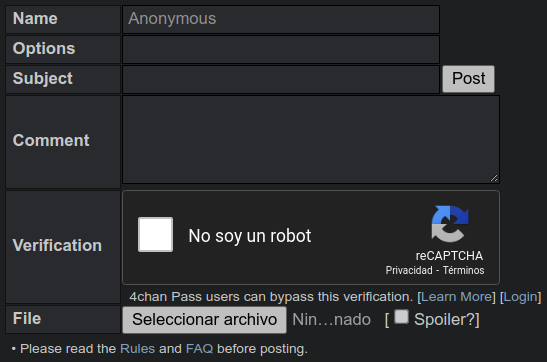
\includegraphics[width=0.7\textwidth]{media/4chan-new-thread.png}
    \end{figure}

    \lstinputlisting[language=Java, style=javastyle, caption=Obtengo la lista de \textit{threads} que hay en un \textit{board}, label=getBoardThreads]{code/getBoardThreads.js}

    \newpage

    % - índice de bloques de código
    \lstlistoflistings
    % para listar esta sección en el tableofcontents
    \addcontentsline{toc}{section}{Ejemplos de código}
    \newpage

    % - bibliografía
    \printbibliography
    % para listar esta sección en el tableofcontents
    \addcontentsline{toc}{section}{Referencias}

\end{document}
